\chapter{जाति-उद्भव और महाविकास}\label{ch:b2:speciation}

गैलापागोस के किसी छोटे द्वीप पर, 1982 में, बड़ी चोंच वाले कुछ
भू-फ़िंच किसी पड़ोसी द्वीप से आए और टिक गए।
बीस वर्ष तक वे उन बड़े \omterm{def:b2:angiosperm-reproduction:seed}{बीजों} के लिए स्थानीय मध्यम भू-फ़िंच से
होड़ करते रहे जो दोनों को भाते थे; फिर कोई सूखा पड़ा, वे
बड़े \omterm{def:b2:angiosperm-reproduction:seed}{बीज} कम पड़ गए, और बड़ी चोंचों वाले स्थानीय ---
यानी वे जो उन नवागंतुकों से सबसे सीधे होड़ करते थे --- भूखे मर गए।
एक ही पीढ़ी के भीतर उन स्थानीयों की चोंचें, मापने लायक ढंग से, उन
हमलावरों की चोंचों से दूर सिकुड़ गईं। दो जातियाँ जो मिली थीं वे
अलग धकेल दी गईं। यह अध्याय जातियों के बनने के बारे में है: कोई जाति
क्या है और उसे भिन्न क्या रखता है, कोई एक समष्टि दो कैसे बनती है, वह
होड़ जो मिलने पर समष्टियों को अलग चलाती है, और जीवाश्म-अभिलेख का
लंबा दृश्य, जहाँ वही प्रक्रिया करोड़ बार दोहराई जाकर जीवन का वृक्ष देती है।

\section{जाति है क्या}

\begin{definition}[जाति]\label{def:b2:speciation:species}
\index{जाति की संकल्पना}\index{जैविक जाति संकल्पना}\index{जननिक विलगन}
\emph{जैविक जाति संकल्पना} के अधीन कोई जाति ऐसी समष्टियों का समूह है
जिनके सदस्य आपस में प्रजनन करके
उर्वर संतति बना सकते हैं, और दूसरे ऐसे समूहों से \emph{जननिक रूप से विलगित}
हैं: जो किसी जाति को जोड़ता है वह \omterm{prop:b2:population-genetics:migration}{जीन-प्रवाह} है, और
जो जातियों को अलग करता है वह उसका अभाव। वह संकल्पना एक ही समय तथा स्थान के
लैंगिक जीवों के लिए चलती है, और अधिकांश वही है जो कोई
जीवविज्ञानी मिलता है; वह अलैंगिक वंशक्रमों के लिए चूक जाती है (जिनके नाम
समानता से रखे जाते हैं), जीवाश्मों के लिए (जिन्हें संकरित नहीं किया जा सकता), और उन
बहुत-सी स्थितियों के लिए जहाँ वह सीमा रिसती है --- बलूत तथा विलो जो
जातियों के आरपार संकरित होते हैं, बत्तख़ें जिनकी जातियाँ बंदी में प्रजनन कर लेती हैं,
और वलय-जातियाँ जिनमें पड़ोसी समष्टियाँ
किसी बाधा के चारों ओर पूरे रास्ते प्रजनन करती हैं जब तक वे सिरे मिलकर
न करने लगें। दूसरी संकल्पनाएँ वे अंतराल पाटती हैं: \emph{आकारिकीय} जाति
(एक जैसे रूपों का कोई गुच्छ), \emph{जातिवृत्तीय} (सबसे छोटा
पहचान-योग्य वंशक्रम), \emph{पारिस्थितिक} (अपना ही निकेत घेरता कोई
वंशक्रम)। कोई भी ग़लत नहीं है; हर एक कुछ असली मापती है, और
जाति-उद्भव वह प्रक्रिया है जिससे वे सहमत होने लगती हैं।
\end{definition}

\begin{proposition}[विलगन-क्रियाविधियाँ]\label{prop:b2:speciation:isolation}
\index{विलगन-क्रियाविधि}\index{पूर्वयुग्मनजी विलगन}\index{पश्चयुग्मनजी विलगन}\index{हैल्डेन का नियम}
दो समष्टियों के बीच \omterm{prop:b2:population-genetics:migration}{जीन-प्रवाह} ऐसी बाधाओं से रुकता है जो
निषेचन से पहले या बाद काम करें। \emph{पूर्वयुग्मनजी}: वे समष्टियाँ
भिन्न आवासों में रहती हैं या भिन्न ऋतुओं में प्रजनन करती हैं (कालिक
विलगन: भिन्न महीनों में पुकारते दो मेंढक); वे एक-दूसरे की
प्रणय-क्रिया नहीं पहचानतीं (व्यवहारिक: झींगुरों के गान,
जुगनुओं के प्रकाश-कूट, बत्तख़ों के नृत्य); उनके
जननांग या \omterm{def:b2:angiosperm-reproduction:flower}{पुष्प} नहीं बैठते (यांत्रिक); उनके युग्मक नहीं
जुड़ते (युग्मकीय: समुद्री अर्चिनों के शुक्राणु-बंधन प्रोटीन,
\cref{ch:b2:angiosperm-reproduction} के $S$ \omterm{def:b2:meiosis-heredity:vocabulary}{युग्मविकल्पी})।
\emph{पश्चयुग्मनजी}: वह संकर भ्रूण के रूप में मर जाता है, या जीता है पर
बंध्य है (खच्चर; दो \emph{Drosophila} जातियों के संकर), या
उर्वर है पर उसकी अपनी संतति नहीं (संकर-भंग)।
\emph{\omterm{prop:b2:speciation:isolation}{हैल्डेन का नियम}}: जब किसी संकर का केवल एक लिंग बंध्य या
अजीवनक्षम हो, तब वह वही लिंग है जिसके दो भिन्न लिंग-गुणसूत्र हैं --- यानी
स्तनियों तथा मक्खियों में नर, और पक्षियों तथा तितलियों में मादा ---
क्योंकि X पर \omterm{def:b2:meiosis-heredity:vocabulary}{अप्रभावी} असंगतियाँ उसी में उघड़ती हैं।
पूर्वयुग्मनजी बाधाएँ सस्ती हैं, क्योंकि कोई युग्मक व्यर्थ नहीं जाते, और
वरण उन्हें वहाँ बनाता है जहाँ पश्चयुग्मनजी पहले से हों।
\end{proposition}

\begin{theorem}[संकर क्यों चूकते हैं: दो-स्थल प्रतिरूप]\label{thm:b2:speciation:dm}
\index{डोब्ज़ान्स्की--म्यूलर असंगति}
दो समष्टियाँ \omterm{def:b2:meiosis-heredity:vocabulary}{जीन-प्ररूप} $aabb$ से शुरू होती हैं। एक में $a$ की जगह
$A$ आ जाता है; दूसरी में $b$ की जगह $B$; और हर प्रतिस्थापन अपनी ही
पृष्ठभूमि में उदासीन या अनुकूल है, इसलिए कोई भी समष्टि कभी किसी कम अनुकूल दशा से
नहीं गुज़रती। पर $A$ तथा $B$ कभी साथ नहीं जाँचे गए, और
यदि वह संयोजन असंगत हो --- यदि $A$ जो प्रोटीन बनाता है वह $B$ के बनाए
प्रोटीन के साथ काम न कर सके --- तो वह संकर $AaBb$ अनुपयुक्त है। इस तरह
\omterm{def:b2:speciation:species}{जननिक विलगन} विचलन के किसी उपोत्पाद के रूप में उपजता है, बिना कोई घाटी पार किए और बिना
स्वयं विलगन के लिए किसी वरण के; और चूँकि किसी एक वंशक्रम में हर नया प्रतिस्थापन
दूसरे में पहले से नियत हर प्रतिस्थापन से असंगत हो सकता है, इसलिए संभव
असंगतियों की संख्या प्रतिस्थापनों की संख्या के \emph{वर्ग} की तरह
बढ़ती है --- यानी विलगन समय के साथ \emph{हिमगोले की तरह बढ़ता} है।
\end{theorem}
\begin{proof}
हर वंशक्रम में $n$ प्रतिस्थापनों के साथ, एक वंशक्रम के $n$ नए युग्मविकल्पियों में से
हर एक दूसरे के $n$ में से हर एक से असंगत हो सकता है:
यानी $n^{2}$ जोड़े, और हर एक किसी प्रायिकता
$\varepsilon$ से असंगत, इसलिए असंगतियों की प्रत्याशित संख्या
$\varepsilon n^{2}$ है, और $n$ उस विभाजन के बाद के समय के साथ बढ़ता है।
वह संकर एकमात्र \omterm{def:b2:meiosis-heredity:vocabulary}{जीन-प्ररूप} है जिसमें वे दोनों समुच्चय मिलते हैं।
\end{proof}
\begin{proof}[प्रमाण-सामग्री]
कोयन और ऑर (1989, 1997) ने ज्ञात आनुवंशिक दूरी (यानी
विचलन के बाद के समय का कोई माप) वाली \emph{Drosophila} जातियों के सैकड़ों
जोड़े संकलित किए और उनका पूर्वयुग्मनजी तथा
\omterm{prop:b2:speciation:isolation}{पश्चयुग्मनजी विलगन} मापा: दोनों उस दूरी के साथ चढ़ते हैं, विलगन
कुछ करोड़ वर्षों के अनुरूप किसी दूरी पर
मूलतः पूरा है, और जो जोड़े एक ही क्षेत्र में रहते हैं वे किसी दी गई दूरी पर
उनसे अधिक \omterm{prop:b2:speciation:isolation}{पूर्वयुग्मनजी विलगन} दिखाते हैं जो नहीं रहते ---
यानी प्रबलन का हस्ताक्षर। तब से असंगति-जीन एक-एक करके
पहचाने गए हैं, और दो जातियों के बीच मिली संख्या उनके विचलन के साथ
रैखिक से तेज़ ही बढ़ती है।
\end{proof}

\begin{omfigure}
\begin{tikzpicture}[every node/.style={font=\scriptsize}, >=stealth]
  \node[draw, rounded corners, fill=omExo!25] (anc) at (0,0) {पूर्वज $aabb$};
  \node[draw, rounded corners, fill=omDef!15] (p1) at (-2.6,-1.8) {समष्टि 1: $AAbb$};
  \node[draw, rounded corners, fill=omThm!15] (p2) at (2.6,-1.8) {समष्टि 2: $aaBB$};
  \node[draw, rounded corners, fill=gray!25, align=center] (hyb) at (0,-3.6) {संकर $AaBb$:\\$A$ और $B$ पहली बार मिलते हैं\\--- असंगत, अनुपयुक्त};
  \draw[->, thick] (anc) -- (p1) node[midway, left, align=right] {$a \to A$ नियत,\\अपनी पृष्ठभूमि में अनुकूल};
  \draw[->, thick] (anc) -- (p2) node[midway, right, align=left] {$b \to B$ नियत,\\अपनी पृष्ठभूमि में अनुकूल};
  \draw[->, thick] (p1) -- (hyb); \draw[->, thick] (p2) -- (hyb);
  \node[anchor=west, align=left, text width=4.6cm] at (4.6,-0.4) {किसी भी समष्टि ने कोई घाटी पार नहीं की; विलगन कोई उपोत्पाद है, और ऐसे जोड़ों की संख्या $n^{2}$ की तरह बढ़ती है};
\end{tikzpicture}

{\small संकर-विफलता का दो-स्थल प्रतिरूप। हर समष्टि कोई ऐसा
परिवर्तन नियत करती है जो उसकी अपनी पृष्ठभूमि में चलता है; और वह संकर पहला
\omterm{def:b2:meiosis-heredity:vocabulary}{जीन-प्ररूप} है जो उन दोनों को जोड़ता है।}
\end{omfigure}

\section{कोई एक जाति दो कैसे बनती है}

\begin{proposition}[जाति-उद्भव के प्रकार]\label{prop:b2:speciation:modes}
\index{भिन्नक्षेत्रीय जाति-उद्भव}\index{समक्षेत्रीय जाति-उद्भव}\index{परिक्षेत्रीय जाति-उद्भव}\index{संस्थापक प्रभाव}
\emph{भिन्नक्षेत्रीय} जाति-उद्भव किसी भौगोलिक बाधा से शुरू होता है:
यानी उठते किसी पर्वत, सूखते किसी सागर या किसी नई नदी से बँटा कोई परास
(\emph{विभंजन}), या किसी द्वीप तक ढोए गए कुछ उपनिवेशी
(\emph{परिधीय}, जिसमें \cref{ch:b2:population-genetics} का
\omterm{prop:b2:speciation:modes}{संस्थापक प्रभाव} तथा अपवाह भी मिले हों)। \omterm{prop:b2:population-genetics:migration}{जीन-प्रवाह} से कट जाने पर
वे दोनों समष्टियाँ भिन्न पर्यावरणों में वरण से,
अपवाह से तथा अपने अलग-अलग \omterm{def:b2:genome-diversification:mutation}{उत्परिवर्तनों} से विचलित होती हैं, जब तक असंगतियाँ
जमा न हो जाएँ; और यदि वे फिर मिलें तो वे अब घुलती नहीं। वह
सबसे आम प्रकार है, और हर स्थलडमरूमध्य, पर्वत-शृंखला तथा जलडमरूमध्य के दोनों
पार्श्वों पर सहोदर जातियों का प्ररूप उसका अभिलेख है।
\emph{समक्षेत्रीय} जाति-उद्भव किसी बाधा के बिना होता है: एक ही चरण में
\omterm{def:b2:genome-diversification:polyploidy}{बहुगुणिता} से (\cref{ch:b2:genome-diversification}) --- पादप जातियों का
एक तिहाई इसी तरह उपजा; या विसमजातीय प्रजनन सहित विदारक वरण से,
जब कोई समष्टि दो संसाधन काम में ले और
व्यष्टि उसी संसाधन पर प्रजनन करें जिसे वे काम में लेते हैं (वह सेब-कीट मक्खी
जो 1860 के दशक में नागफनी से सेब पर खिसकी और अब
अपने परपोषी पर प्रजनन करती है; किसी क्रेटर-झील की सिक्लिड)। \emph{परिक्षेत्रीय}
जाति-उद्भव किसी पर्यावरणीय प्रवणता के साथ होता है, जहाँ कोई
समष्टि दोनों सिरों के अनुरूप ढलती है और बीच में कोई \omterm{prop:b2:speciation:reinforcement}{संकर-क्षेत्र}
बनता है। हर प्रकार में वह नुस्ख़ा वही है: \omterm{prop:b2:population-genetics:migration}{जीन-प्रवाह} घटाइए,
विचलन को जमा होने दीजिए, और विचलन के उपोत्पादों को
बाधाएँ बन जाने दीजिए।
\end{proposition}

\begin{omfigure}
\resizebox{\linewidth}{!}{%
\begin{tikzpicture}[every node/.style={font=\scriptsize}, >=stealth]
  \foreach \x/\lab in {0/{भिन्नक्षेत्रीय:\\कोई बाधा उस परास को बाँटती है}, 5.2/{परिधीय:\\किसी द्वीप पर कुछ संस्थापक}, 10.4/{समक्षेत्रीय:\\दो परपोषी, परपोषी पर प्रजनन}} \node[align=center, anchor=south] at (\x+1.8,3.0) {\lab};
  % allopatric
  \draw[thick, fill=omDef!15] (0.9,1.4) ellipse (0.8 and 0.9);
  \draw[thick, fill=omThm!15] (2.7,1.4) ellipse (0.8 and 0.9);
  \draw[very thick, omExo!70!black] (1.8,0.2) -- (1.8,2.6);
  \node[below] at (1.8,0.1) {पर्वत, सागर, नदी};
  % peripatric
  \begin{scope}[xshift=5.2cm]
    \draw[thick, fill=omDef!15] (1.0,1.4) ellipse (1.0 and 0.9);
    \draw[thick, fill=omThm!15] (3.2,1.9) circle (0.35);
    \draw[->, thick, dashed] (2.0,1.6) -- (2.85,1.85);
    \node[below] at (3.2,1.5) {संस्थापक};
    \node[below] at (1.0,0.4) {मुख्यभूमि};
  \end{scope}
  % sympatric
  \begin{scope}[xshift=10.4cm]
    \draw[thick, fill=omExo!15] (1.8,1.4) ellipse (1.7 and 0.9);
    \foreach \p in {(1.0,1.6),(1.3,1.2),(0.8,1.2),(1.2,1.8)} \fill[omDef] \p circle (0.07);
    \foreach \p in {(2.4,1.6),(2.7,1.2),(2.2,1.2),(2.6,1.8)} \fill[omThm] \p circle (0.07);
    \node[omDef, below] at (1.0,0.5) {परपोषी A}; \node[omThm, below] at (2.6,0.5) {परपोषी B};
    \node[below] at (1.8,0.1) {एक जगह, दो संसाधन};
  \end{scope}
\end{tikzpicture}}

{\small दो जातियों तक तीन रास्ते: उस परास के आरपार कोई बाधा, उसके परे कोई
संस्थापक समष्टि, या उसके भीतर दो संसाधन।}
\end{omfigure}

\begin{proposition}[प्रबलन और संकर-क्षेत्र]\label{prop:b2:speciation:reinforcement}
\index{प्रबलन}\index{संकर-क्षेत्र}\index{क्लाइन}
जब दो विचलित समष्टियाँ फिर मिलती हैं, तब तीन बातें हो सकती हैं।
यदि उनके संकर जनकों जितने ही अनुकूल हों, तो वे घुल जाती हैं। यदि वे
संकर अनुपयुक्त हों, तो वरण उन व्यष्टियों को अनुकूल पाता है जो दूसरी क़िस्म से
प्रजनन करने से इनकार करें --- और व्यर्थ गए युग्मक ही वह दाम हैं --- तथा
जहाँ वे दोनों अतिव्यापित हों वहाँ \omterm{prop:b2:speciation:isolation}{पूर्वयुग्मनजी विलगन} मज़बूत होता है
(यानी \emph{प्रबलन}), जब तक वे जातियाँ न हो जाएँ। इनके बीच कोई
\emph{\omterm{prop:b2:speciation:reinforcement}{संकर-क्षेत्र}} बना रहता है: यानी कोई पट्टी, अक्सर कुछ किलोमीटर चौड़ी,
जहाँ वे दोनों रूप आपस में प्रजनन करते हैं और हर पीढ़ी संकर बनते हैं,
और जो उस क्षेत्र में प्रकीर्णन तथा उसके भीतर संकरों के विरुद्ध वरण के
संतुलन से बनी रहती है। ऐसे किसी क्षेत्र के आरपार
हर रूप की बारंबारता किसी \emph{क्लाइन} पर चलती है, यानी कोई S-आकार का
वक्र जिसकी चौड़ाई $w$ प्रति पीढ़ी प्रकीर्णन-दूरी $\sigma$
और संकरों के विरुद्ध वरण $s$ से बैठती है, $w \approx
\sigma\sqrt{8/s}$: और कोई क्षेत्र हज़ारों वर्ष सँकरा रह सकता है
बिना उन दोनों रूपों के कभी जुड़े या पूरी तरह अलग हुए। यूरोप के मेंढक,
कौवे, चूहे तथा टिड्डे उनके दर्जनों दिखाते हैं, जिनमें अधिकांश उन रेखाओं पर
चलते हैं जहाँ पिछले हिमयुग में अलग-अलग शरणों में पनाह लिए समष्टियाँ
हिम के हटते ही फिर मिलीं।
\end{proposition}
\begin{proof}[प्रमाण-सामग्री]
जहाँ मध्य यूरोप में चितकबरी तथा कंठी मक्खीमार अतिव्यापित हैं,
वहाँ हर जाति के नरों का पंखावरण दूसरे से उससे अधिक भिन्न है
जितना वहाँ जहाँ वे अलग रहते हैं, और मादाएँ अधिक तीखे ढंग से
भेद करती हैं --- यानी खेत में मापा गया प्रबलन। अग्नि-उदर तथा
पीत-उदर मेंढक पोलैंड के आरपार कुछ किलोमीटर चौड़े किसी क्षेत्र के साथ
मिलते हैं, जो जब से अध्ययन हुआ है तब से स्थिर है, और
उनके प्रकीर्णन तथा उनके संकरों की घटी \omterm{def:b2:population-genetics:fitness}{अनुकूलता} से
क्लाइन-चौड़ाई बताई जा चुकी है।
\end{proof}

\begin{omfigure}
\begin{tikzpicture}
\begin{axis}[
  width=0.72\linewidth, height=5.2cm,
  axis x line=bottom, axis y line=left,
  xmin=-30, xmax=30, ymin=0, ymax=1.05,
  xlabel={उस क्षेत्र के आरपार दूरी (km)}, ylabel={रूप A की बारंबारता},
  xlabel style={font=\small, at={(axis description cs:0.5,-0.13)}, anchor=north},
  ylabel style={font=\small},
  tick label style={font=\small}, xtick={-20,-10,0,10,20}, ytick={0,0.5,1},
  clip=false,
]
\addplot[very thick, omDef, domain=-30:30, samples=100] {1/(1+exp(x/2.2))};
\draw[dashed, gray] (axis cs:-4.4,0) -- (axis cs:-4.4,1); \draw[dashed, gray] (axis cs:4.4,0) -- (axis cs:4.4,1);
\draw[<->] (axis cs:-4.4,0.08) -- (axis cs:4.4,0.08); \node[font=\scriptsize, anchor=south] at (axis cs:0,0.09) {चौड़ाई $w$};
\node[font=\scriptsize, anchor=west, align=left] at (axis cs:8,0.75) {$w \approx \sigma\sqrt{8/s}$: प्रकीर्णन\\$\sigma = \qty{1}{km}$, $s = 0.1$\\से $w \approx \qty{9}{km}$};
\end{axis}
\end{tikzpicture}

{\small किसी \omterm{prop:b2:speciation:reinforcement}{संकर-क्षेत्र} के आरपार कोई क्लाइन: किसी एक रूप की बारंबारता
एक से शून्य तक ऐसी चौड़ाई भर गिरती है जो इससे बैठती है कि व्यष्टि कितनी दूर
प्रकीर्ण होते हैं और उनके संकर कितने अनुपयुक्त हैं।}
\end{omfigure}

\section{होड़, सहअस्तित्व और लक्षण-विस्थापन}

\begin{theorem}[लॉटका--वोल्तेरा होड़]\label{thm:b2:speciation:lv}
\index{लॉटका--वोल्तेरा होड़}\index{होड़ से अपवर्जन}\index{सहअस्तित्व}
लॉजिस्टिक वृद्धि (वर्ष 1 का खंड) वाली दो जातियाँ जो किसी
संसाधन के लिए होड़ करें, ये मानती हैं:
\[
\frac{\mathrm{d}N_1}{\mathrm{d}t} = r_1 N_1\Bigl(1 - \frac{N_1 + \alpha N_2}{K_1}\Bigr), \qquad
\frac{\mathrm{d}N_2}{\mathrm{d}t} = r_2 N_2\Bigl(1 - \frac{N_2 + \beta N_1}{K_2}\Bigr),
\]
जिसमें $\alpha$ जाति 2 के एक व्यष्टि का जाति 1 पर प्रभाव
जाति 1 के अपने व्यष्टियों की इकाइयों में मापता है, और $\beta$
उलटा। जाति 1 रेखा $N_1 + \alpha N_2 =
K_1$ पर बढ़ना रोक देती है (यानी उसका \emph{समरेख}), जाति 2 $N_2 + \beta N_1 = K_2$ पर, और
वह परिणाम इस पर निर्भर है कि वे दोनों रेखाएँ कैसे काटती हैं:
\begin{itemize}
  \item $K_1 > \alpha K_2$ तथा $K_2 < \beta K_1$: जाति 1 सदा
        जीतती है;
  \item $K_1 < \alpha K_2$ तथा $K_2 > \beta K_1$: जाति 2 सदा
        जीतती है;
  \item $K_1 > \alpha K_2$ तथा $K_2 > \beta K_1$: $N_1^{*} = (K_1 - \alpha K_2)/(1 - \alpha\beta)$,
        $N_2^{*} = (K_2 - \beta K_1)/(1 - \alpha\beta)$ पर \emph{स्थिर
        सहअस्तित्व};
  \item $K_1 < \alpha K_2$ तथा $K_2 < \beta K_1$: कोई भी जीतता है,
        इस पर निर्भर कि कौन अधिक संख्या से शुरू करे।
\end{itemize}
सहअस्तित्व को $\alpha\beta < 1$ चाहिए, और हर जाति को अपनी ही क़िस्म से
दूसरी से अधिक रोका जाना चाहिए: जो दो जातियाँ ठीक वही संसाधन काम में लें
($\alpha = \beta = 1$) वे सह-अस्तित्व में नहीं रह सकतीं
(यानी \emph{\omterm{thm:b2:speciation:lv}{होड़ से अपवर्जन} का सिद्धांत}), और वे जो काम में लेती हैं उसमें जितना
अधिक भिन्न हों, उतने ही छोटे $\alpha$ तथा $\beta$ और उतनी ही
सुरक्षित उनकी सह-उपस्थिति।
\end{theorem}
\begin{proof}
जाति 1 के समरेख पर $\mathrm{d}N_1/\mathrm{d}t = 0$; उससे नीचे
(मूल बिंदु की ओर) $N_1$ बढ़ता है, उससे ऊपर $N_1$ गिरता है; और वैसे ही
जाति 2 के लिए। हर समरेख कोई सरल रेखा है जिसके अंतःखंड $K_1$ ($N_1$ अक्ष पर)
और $K_1/\alpha$ ($N_2$ अक्ष पर) हैं (जाति 1 के),
तथा $K_2/\beta$ और $K_2$ (जाति 2 के)। जाति 1 जाति 2 की किसी ऐसी समष्टि पर
आक्रमण कर सकती है जो अपनी धारण-क्षमता $K_2$ पर हो, यदि वहाँ उसकी अपनी
वृद्धि धनात्मक हो, यानी यदि $K_1 > \alpha K_2$; और जाति 2 जाति 1 पर $K_1$ पर
आक्रमण कर सकती है यदि $K_2 > \beta K_1$। जब दोनों दूसरे पर आक्रमण कर सकें,
तब किसी को अपवर्जित नहीं किया जा सकता और वे प्रक्षेप-पथ उन समरेखों के
कटान पर अभिसरित होते हैं, जो उन दो रेखा-समीकरणों को हल करके मिलता है;
जब केवल एक कर सके, तब वही जीतती है; और जब कोई भी न कर सके, तब वह
कटान कोई काठी है और संस्थापक जीतता है। उस भीतरी बिंदु की स्थिरता
उसी आक्रमण-तर्क से निकलती है: किसी भी अक्ष की ओर विक्षुब्ध किए जाने पर
दुर्लभ जाति फिर बढ़ आती है।
\end{proof}

\begin{omfigure}
\begin{tikzpicture}
\begin{axis}[
  width=0.6\linewidth, height=6cm,
  axis x line=bottom, axis y line=left,
  xmin=0, xmax=1300, ymin=0, ymax=1900,
  xlabel={$N_1$}, ylabel={$N_2$},
  xlabel style={font=\small, at={(axis description cs:0.5,-0.1)}, anchor=north},
  ylabel style={font=\small},
  tick label style={font=\small}, xtick={0,857,1000,1333}, xticklabels={0,$N_1^*$,$K_1$,$K_2/\beta$}, ytick={0,286,800,2000}, yticklabels={0,$N_2^*$,$K_2$,$K_1/\alpha$},
  clip=false,
]
\addplot[very thick, omDef, domain=50:1000, samples=2] {(1000-x)/0.5};
\addplot[very thick, omThm, domain=0:1333, samples=2] {800-0.6*x};
\fill[black] (axis cs:857,286) circle (2.5pt);
\draw[->, thick, gray] (axis cs:150,1750) -- (axis cs:300,1450);
\draw[->, thick, gray] (axis cs:1200,100) -- (axis cs:1000,250);
\draw[->, thick, gray] (axis cs:150,150) -- (axis cs:400,250);
\node[font=\scriptsize, omDef, anchor=west] at (axis cs:700,1000) {जाति 1 का समरेख};
\node[font=\scriptsize, omThm, anchor=south west] at (axis cs:130,740) {जाति 2 का समरेख};
\node[font=\scriptsize, anchor=south west] at (axis cs:880,320) {स्थिर सहअस्तित्व};
\end{axis}
\end{tikzpicture}

{\small $K_1 = 1000$, $K_2 =
800$, $\alpha = 0.5$, $\beta = 0.6$ वाले दो होड़ियों का कला-तल: हर जाति दूसरी की
धारण-क्षमता पर आक्रमण कर सकती है, और वे प्रक्षेप-पथ
$N_1^{*} = 857$, $N_2^{*} = 286$ पर समरेखों के कटान पर अभिसरित होते हैं।}
\end{omfigure}

\begin{proposition}[लक्षण-विस्थापन]\label{prop:b2:speciation:displacement}
\index{लक्षण-विस्थापन}\index{निकेत}\index{अनुकूली विकिरण}
होड़ केवल कोई पारिस्थितिक परिणाम नहीं बल्कि कोई विकासीय
बल भी है। जहाँ दो एक जैसी जातियाँ मिलें, वहाँ हर एक के वे व्यष्टि
जो दूसरी से सबसे अधिक मिलते हैं उस होड़ से सबसे अधिक भोगते हैं, और
वरण उन दोनों को उस लक्षण में अलग धकेलता है जो
संसाधन-उपयोग बाँधता है --- चोंच का आकार, देह का आकार, पुष्पन-काल: यानी वे
समष्टियाँ जो अतिव्यापित हों उनसे अधिक भिन्न होती हैं जो अकेली
रहती हैं। यह \emph{लक्षण-विस्थापन} $\alpha$ तथा
$\beta$ को सिकोड़ता है, अपवर्जन की किसी होड़ को सहअस्तित्व में बदल देता है, और,
अवसरों के किसी भूदृश्य भर दोहराया जाए तो, कोई
\emph{\omterm{prop:b2:speciation:displacement}{अनुकूली विकिरण}} पैदा करता है: यानी कोई एक उपनिवेशी दर्जन भर जातियाँ बनता
जिनमें हर एक किसी संसाधन के अनुरूप हो --- गैलापागोस पर डार्विन के फ़िंच,
हवाई के हनीक्रीपर, अफ़्रीकी झीलों की सिक्लिड
(पंद्रह हज़ार वर्ष से भी कम में विक्टोरिया झील में पाँच सौ जातियाँ),
कैरिबियन की एनोल छिपकलियाँ, जहाँ निकेतों का वही समुच्चय
देह-रूपों के उसी समुच्चय से चार द्वीपों पर स्वतंत्र रूप से भर दिया गया है।
\end{proposition}
\begin{proof}[प्रमाण-सामग्री]
ग्रांट दंपति ने डैफ़्नी मेजर पर चालीस वर्ष तक हर फ़िंच अभिलिखित किया।
1982 में बड़े भू-फ़िंच के जम जाने के बाद
मध्यम भू-फ़िंच की चोंच 2004 के सूखे तक नहीं बदली,
जब बड़े \omterm{def:b2:angiosperm-reproduction:seed}{बीज} दुर्लभ हो गए और वे दोनों जातियाँ उनके लिए होड़ करने
लगीं; सबसे बड़ी चोंचों वाले मध्यम फ़िंच असमानुपाती ढंग से मरे,
और अगली पीढ़ी की चोंचें उससे अधिक छोटी थीं जितना
किसी एक ही चरण में कभी देखा गया था --- यानी सिद्धांत से बताया गया
लक्षण-विस्थापन, घटते हुए देखा गया, और उसका
वरण अंतर तथा वंशागतिता मापी गई। उन्हीं फ़िंचों की चोंचें,
उन द्वीपों के बीच तुलना की जाएँ जहाँ वे अकेले रहते हैं और जिन
द्वीपों पर वे मिलते हैं, वही विस्थापन उस द्वीपसमूह भर लिखा दिखाती हैं।
\end{proof}

\begin{omfigure}
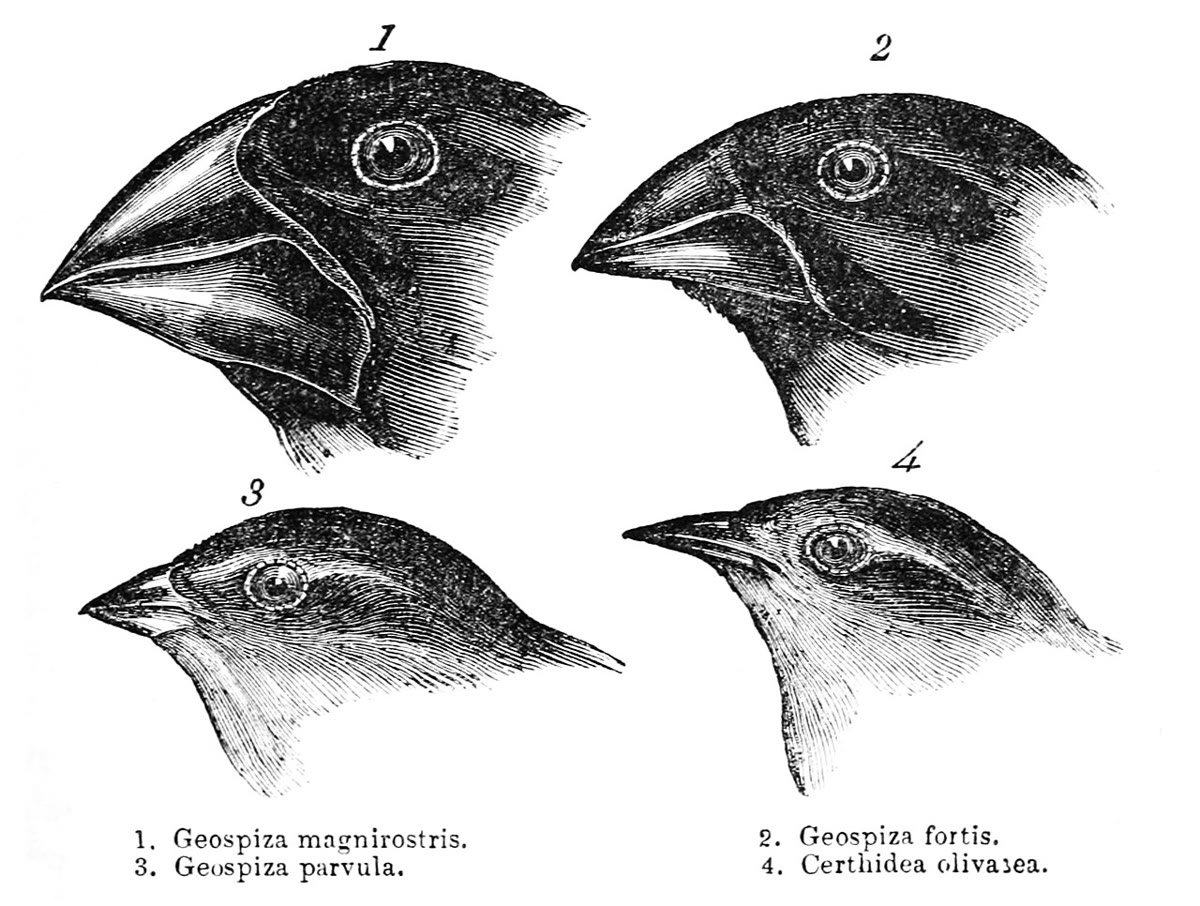
\includegraphics[width=0.44\linewidth]{images/book2/finches-gould.jpg}\hspace{0.04\linewidth}
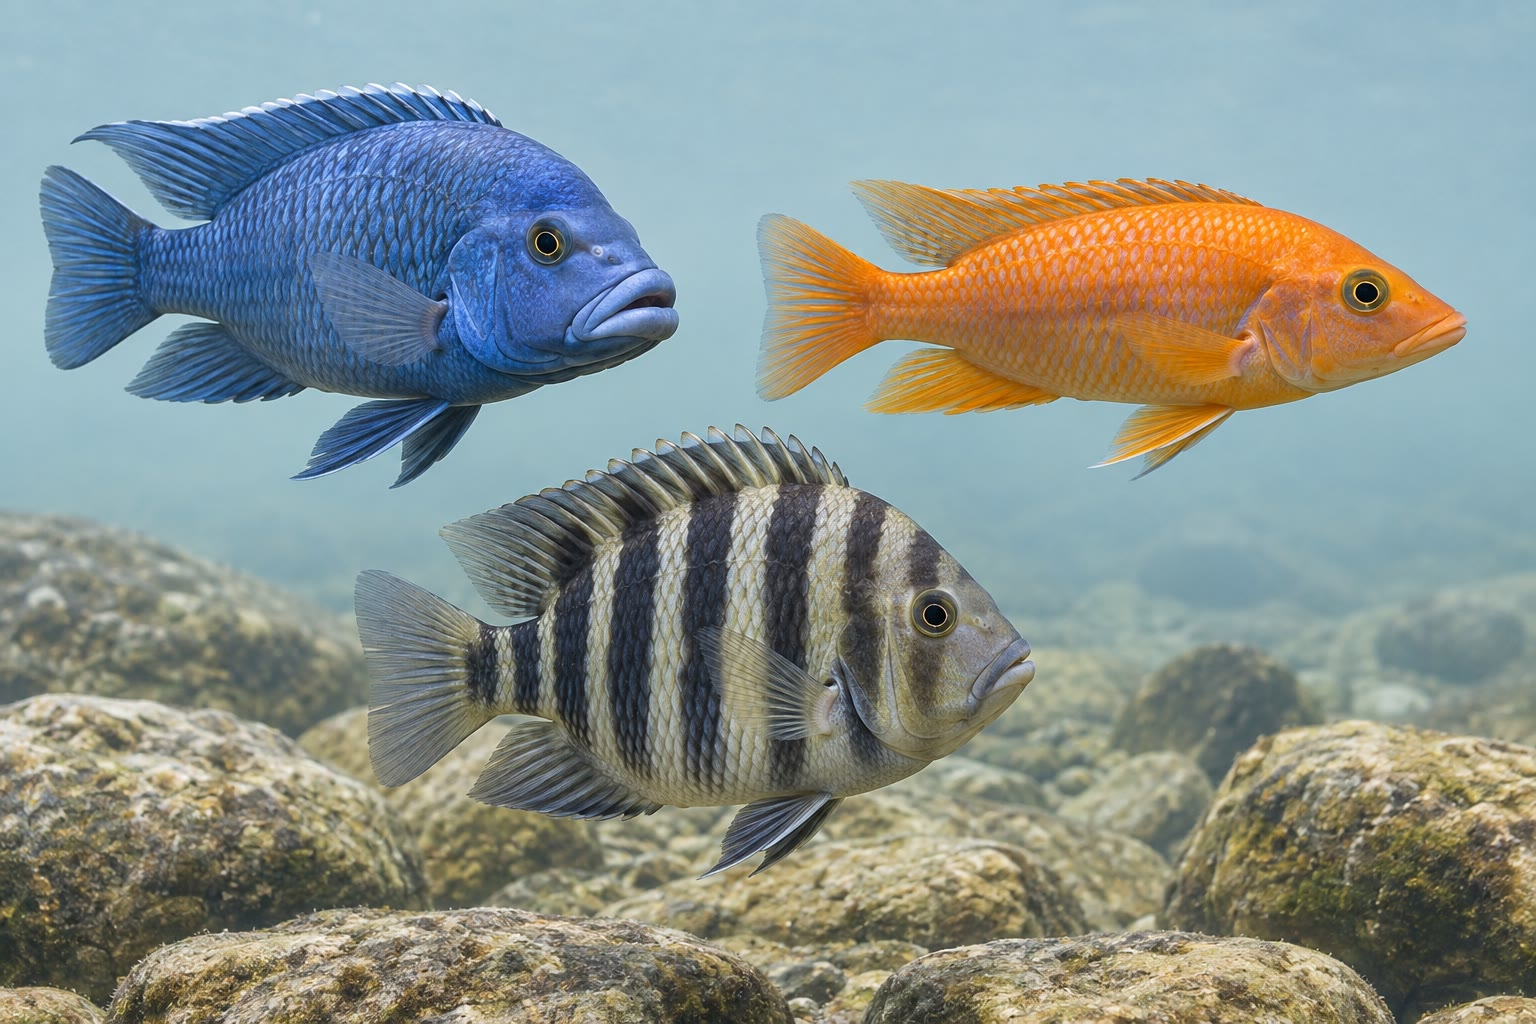
\includegraphics[width=0.44\linewidth]{images/book4/ai/b4-23-cichlids.jpg}

{\small दो विकिरण। बाएँ: 1845 में गूल्ड के खींचे डार्विन के फ़िंच,
यानी कोई एक उपनिवेशी बहुत बना, जो अपनी चोंचों से पहचाने जाते हैं।
दाएँ: किसी अफ़्रीकी झील की सिक्लिड, कुछ संस्थापकों से सैकड़ों जातियाँ,
हर एक अपने ही मुँह तथा आहार के साथ।}
\end{omfigure}

\section{महाविकास: लंबा दृश्य}

\begin{proposition}[गति और प्रकार]\label{prop:b2:speciation:tempo}
\index{विरामित साम्य}\index{क्रमिकतावाद}\index{सामूहिक विलोपन}
कुछ दर्जन पीढ़ियों में उस पतंगे ने रंग बदला और उस फ़िंच ने
अपनी चोंच; और करोड़ों वर्षों में जीवाश्म-अभिलेख ऐसे वंशक्रम दिखाता है
जो लंबे-लंबे खंडों तक मुश्किल से बदलते हैं और फिर, कुछ हज़ार वर्षों के किसी
भूवैज्ञानिक क्षण में, किसी भिन्न वंशज से बदल दिए जाते हैं
--- यानी \emph{\omterm{prop:b2:speciation:tempo}{विरामित साम्य}}, और छोटी परिधीय समष्टियों में
\omterm{prop:b2:speciation:modes}{भिन्नक्षेत्रीय जाति-उद्भव} के बाद उनका फैलाव हर लाख वर्ष पर
प्रतिचयित किए जाने पर ऐसा ही दिखता है;
और वह दूसरे वंशक्रम भी दिखाता है, जिनमें घोड़े भी हैं, जो दर्जनों जातियों भर
क्रमशः बदलते हैं। जाति के ऊपर वह अभिलेख
उलट-फेर का है: अधिकांश जातियाँ दस लाख से एक करोड़ वर्ष चलती हैं,
\emph{पृष्ठभूमि विलोपन} दर प्रति वर्ष दस लाख में लगभग एक
जाति है, और पाँच बार --- ऑर्डोविशी, डिवोनी, पर्मी (जब
समुद्री जातियों के दस में से नौ भाग लुप्त हुए), ट्राइऐसी तथा क्रिटेशी के अंत में ---
किसी \emph{\omterm{prop:b2:speciation:tempo}{सामूहिक विलोपन}} ने कुछ लाख वर्षों के भीतर जो जीता था उसका अधिकांश
हटा दिया और वह खेल फिर से बैठा दिया, और बचे हुए
ख़ाली हुए निकेतों में विकिरित हुए: यानी 6.6 करोड़ वर्ष पहले उस क्षुद्रग्रह के बाद
डायनासोरों की दुनिया में स्तनी। महाविकास वह प्ररूप है जो इस तथा
पिछले अध्याय के सूक्ष्मविकास ने, बहुत लंबे समय तक चलकर और
आपदा से टूटकर, खींचा है।
\end{proposition}

\begin{example}[दरों की तुलना]\label{ex:b2:speciation:rates}
उन फ़िंचों पर वरण ने चोंच की गहराई एक ही पीढ़ी में \qty{4}{\%} बदल दी;
पूरे गैलापागोस विकिरण को, यानी एक संस्थापक से चौदह जातियों को,
बीस लाख वर्ष लगे; किसी चूहे और किसी हाथी के बीच
देह-आकार का अंतर, कोई $10^{5}$, उस फ़िंच जितनी ताक़त के वरण से
कुछ सौ पीढ़ियों में पैदा किया जा सकता था ---
और वह अभिलेख दिखाता है कि उसमें चार करोड़ वर्ष लगे। वह विरोधाभास
यह देखकर सुलझ जाता है कि वरण शायद ही कभी लंबे समय तक उसी ओर धकेलता है:
वह मौसम के साथ उलट जाता है, जैसा उस सूखे के अगले वर्ष डैफ़्नी मेजर पर
हुआ, और \omterm{prop:b2:population-genetics:kinds}{स्थायीकारी वरण} अधिकांश वंशक्रमों को
जहाँ हैं वहीं थामे रखता है। बना रहता परिवर्तन दुर्लभ है, और इसीलिए
जाति-उद्भव, जिसे वह चाहिए, धीमा है --- और इसीलिए, जब वह दुनिया
तेज़ बदलती है, जैसा \cref{ch:b2:global-change} में होता है, तब वे
वंशक्रम खो जाते हैं जो साथ नहीं चल सकते।
\end{example}

\section{अभ्यास}

\begin{exercise}[$\star$]\label{exo:b2:speciation:1}
\omterm{def:b2:speciation:species}{जैविक जाति संकल्पना} बताइए और तीन ऐसी स्थितियाँ दीजिए जिनमें
वह लागू नहीं की जा सकती, और उसके बजाय काम में ली गई संकल्पना।
\end{exercise}

\begin{exercise}[$\star$]\label{exo:b2:speciation:2}
पूर्वयुग्मनजी या पश्चयुग्मनजी के रूप में वर्गीकृत कीजिए: भिन्न महीनों में
प्रजनन करते दो मेंढक; कोई खच्चर; समुद्री अर्चिन का कोई ऐसा शुक्राणु जो
किसी दूसरी जाति के अंड से बँध न सके; ऐसे संकर पौधे जो ओजस्वी हैं पर जिनके
\omterm{def:b2:angiosperm-reproduction:seed}{बीज} अंकुरित नहीं होते; भिन्न गान वाले दो झींगुर।
\end{exercise}

\begin{exercise}[$\star$]\label{exo:b2:speciation:3}
भिन्नक्षेत्रीय, परिधीय, समक्षेत्रीय तथा \omterm{prop:b2:speciation:modes}{परिक्षेत्रीय जाति-उद्भव} की
परिभाषा दीजिए, और हर एक का एक उदाहरण।
\end{exercise}

\begin{exercise}[$\star$]\label{exo:b2:speciation:4}
\omterm{thm:b2:speciation:lv}{लॉटका--वोल्तेरा होड़} के चारों परिणाम और स्थिर सहअस्तित्व की
शर्त शब्दों में बताइए।
\end{exercise}

\begin{exercise}[$\star\star$]\label{exo:b2:speciation:5}
$K_1 = 1000$, $K_2 = 800$, $\alpha = 0.5$, $\beta = 0.6$ के साथ
साम्य घनत्व निकालिए और जाँचिए कि हर जाति दूसरी की धारण-क्षमता पर
आक्रमण कर सकती है।
\end{exercise}

\begin{exercise}[$\star\star$]\label{exo:b2:speciation:6}
$K_1 = 1000$, $K_2 = 800$, $\alpha = 1.5$, $\beta = 0.3$ के साथ कौन-सी
जाति जीतती है, और क्यों? और यदि $\alpha = 1.5$ तथा $\beta = 1.5$ हों तो?
\end{exercise}

\begin{exercise}[$\star\star$]\label{exo:b2:speciation:7}
किसी \omterm{def:b2:meiosis-heredity:meiosis}{द्विगुणित} समष्टि में कोई चतुर्गुणित उपजता है। उसके युग्मकों की, उस
\omterm{def:b2:meiosis-heredity:meiosis}{द्विगुणित} के साथ किसी संकरण की, और उस संकर के युग्मकों की गुणसूत्र-संख्याएँ
दीजिए, और समझाइए कि वह चतुर्गुणित तुरंत क्यों विलगित है। फिर भी वह आम तौर पर
टिकने में क्यों चूक जाता है?
\end{exercise}

\begin{exercise}[$\star\star$]\label{exo:b2:speciation:8}
दो समष्टियों ने अपने विभाजन के बाद हर एक 10 प्रतिस्थापन नियत किए हैं,
और दोनों ओर के नए युग्मविकल्पियों का हर जोड़ा प्रायिकता $0.01$ से
असंगत है। अभी, और हर एक 30 प्रतिस्थापनों के बाद, असंगतियों की
प्रत्याशित संख्या निकालिए। यह समय के साथ विलगन के संबंध के बारे में
क्या बताता है?
\end{exercise}

\begin{exercise}[$\star\star$]\label{exo:b2:speciation:9}
प्रति पीढ़ी प्रकीर्णन $\sigma =
\qty{2}{km}$ तथा संकर-हानि $s = 0.05$ के लिए, और
$\sigma = \qty{0.3}{km}$ तथा $s = 0.4$ के लिए किसी \omterm{prop:b2:speciation:reinforcement}{संकर-क्षेत्र} की चौड़ाई निकालिए। कौन-सा क्षेत्र
प्रबलन में अंत होने की अधिक संभावना रखता है, और क्यों?
\end{exercise}

\begin{exercise}[$\star\star\star$]\label{exo:b2:speciation:10}
दो फ़िंच जातियाँ $\alpha = \beta = 0.9$ तथा
$K_1 = K_2 = 500$ के साथ \omterm{def:b2:angiosperm-reproduction:seed}{बीजों} के लिए होड़ करती हैं। क्या वे सह-अस्तित्व में रहती हैं? लक्षण-विस्थापन
$\alpha$ तथा $\beta$ को $0.4$ कर देता है: साम्य फिर से निकालिए। समरेखों
के हिसाब से समझाइए कि उस विस्थापन ने क्या किया।
\end{exercise}

\begin{exercise}[$\star\star\star$]\label{exo:b2:speciation:11}
ग्रांट दंपति ने पाया कि 2004 के सूखे के बाद मध्यम भू-फ़िंच की
माध्य चोंच-गहराई $h^{2} = 0.7$ के साथ \qty{0.7}{mm} गिरी,
और बचे हुओं की चोंचें उस समष्टि से \qty{1}{mm} छोटी थीं।
\omterm{thm:b2:population-genetics:heritability}{प्रजनक-समीकरण} से वह अनुक्रिया जाँचिए, और
समझाइए कि उस परिवर्तन की दिशा का कारण बड़े भू-फ़िंच की उपस्थिति क्यों थी, केवल वह सूखा नहीं।
\end{exercise}

\begin{exercise}[$\star\star\star$]\label{exo:b2:speciation:12}
``जातियाँ संयोग से बनती हैं और वरण से रखी जाती हैं।'' दो-स्थल प्रतिरूप,
प्रबलन, और भूगोल की भूमिका के साथ इस पर विचार कीजिए।
\end{exercise}

\section{समस्या: किसी द्वीप पर दो फ़िंच}

\begin{problem}[{सप्तांत समस्या --- कोई स्थानीय फ़िंच किसी
हमलावर से मिलता है: उनकी होड़ का कला-तल पर विश्लेषण, उस स्थानीय की चोंच का
विस्थापन प्रजनक-समीकरण से बताया गया, और उनके बीच विलगन किसी
संकर-क्षेत्र के मुक़ाबले मापा गया, और अंत उन साम्य घनत्वों, उस चोंच की खिसक, तथा
उस क्लाइन-चौड़ाई पर}]
\label{pb:b2:speciation:1}
स्थानीय जाति 1: $K_1 = 1200$, $r_1 = 0.5$ प्रति वर्ष; हमलावर
जाति 2: $K_2 = 400$। विस्थापन से पहले $\alpha = 0.9$, $\beta =
0.3$; और कोई सूखा दोनों धारण-क्षमताएँ एक वर्ष के लिए आधी कर देता है। जाति 1 की
चोंच-गहराई: माध्य \qty{9.5}{mm}, मानक विचलन
\qty{0.8}{mm}, $h^{2} = 0.7$। \omterm{prop:b2:speciation:reinforcement}{संकर-क्षेत्र} प्राचल: $\sigma =
\qty{0.5}{km}$, $s = 0.2$।

\medskip
\noindent\textbf{भाग I --- वह आक्रमण।}
\begin{enumerate}
  \item दोनों समरेख और उनके अंतःखंड लिखिए।
  \item क्या जाति 2 जाति 1 पर $K_1$ पर आक्रमण कर सकती है? क्या जाति 1
        जाति 2 पर $K_2$ पर? परिणाम पर निष्कर्ष निकालिए।
  \item साम्य घनत्व निकालिए।
  \item उस क्षण $\mathrm{d}N_1/\mathrm{d}t$ निकालिए जब जाति 2
        $N_2 = 20$ तथा $N_1 = 1200$ के साथ आती है। उसके चिह्न का क्या
        अर्थ है?
  \item उस सूखे में दोनों $K$ आधे हो जाते हैं। वह साम्य फिर से निकालिए
        और कहिए कि हर जाति की संख्या का क्या होता है।
  \item उस स्थानीय पर उस हमलावर का प्रभाव ($\alpha = 0.9$) उस हमलावर पर
        उस स्थानीय के प्रभाव ($\beta = 0.3$) से बड़ा क्यों है?
\end{enumerate}

\medskip
\noindent\textbf{भाग II --- विस्थापन।}
उस सूखे में सबसे बड़ी चोंचों वाले स्थानीय व्यष्टि उस हमलावर से
सबसे अधिक होड़ करते हैं और मर जाते हैं: बचे हुओं की माध्य
चोंच \qty{9.0}{mm} है।
\begin{enumerate}[resume]
  \item वरण अंतर और वह अनुक्रिया निकालिए।
  \item अगली पीढ़ी की माध्य चोंच बताइए।
  \item उस खिसक के बाद $\alpha$ गिरकर $0.5$ हो जाता है। वह साम्य
        फिर से निकालिए (मूल $K$ के साथ)।
  \item समझाइए कि उस खिसक ने जाति 1 के समरेख का क्या किया।
  \item यदि इतनी ताक़त का वरण हर वर्ष काम करे, तो उस चोंच को
        \qty{2}{mm} खिसकाने में कितने वर्ष लगते? वह ऐसा करता
        क्यों नहीं?
  \item उस विकिरण की बीस लाख वर्ष की आयु से तुलना कीजिए और
        टिप्पणी कीजिए।
\end{enumerate}

\medskip
\noindent\textbf{भाग III --- विलगन।}
वे दोनों जातियाँ संकरित हो सकती हैं; संकरों की चोंचें मध्यवर्ती होती हैं और
\omterm{def:b2:population-genetics:fitness}{अनुकूलता} $1 - s$।
\begin{enumerate}[resume]
  \item वह पूर्वयुग्मनजी बाधा बताइए जो डार्विन के फ़िंचों में संकरण
        दुर्लभ रखती है, और उन संकरों की एक पश्चयुग्मनजी
        लागत।
  \item उनके बीच किसी \omterm{prop:b2:speciation:reinforcement}{संकर-क्षेत्र} की चौड़ाई $\sigma
        = \qty{0.5}{km}$, $s = 0.2$ के लिए निकालिए।
  \item वह द्वीप \qty{1}{km} चौड़ा है। उसका क्या अर्थ निकलता है?
  \item समझाइए कि प्रबलन कैसे आगे बढ़ता, और वह किस लक्षण पर
        काम करता।
  \item भिन्न द्वीपों पर उस स्थानीय की दो समष्टियों ने अलग होने के बाद
        हर एक 15 प्रतिस्थापन नियत किए हैं; और जोड़े प्रायिकता $0.005$ से
        असंगत हैं। प्रत्याशित असंगतियाँ निकालिए और कहिए कि वे जातियाँ हैं या नहीं।
  \item क्या \omterm{def:b2:speciation:species}{जैविक जाति संकल्पना}, आकारिकीय
        संकल्पना तथा जातिवृत्तीय संकल्पना उन दोनों द्वीप-समष्टियों के बारे में
        सहमत होतीं? समझाइए।
\end{enumerate}

\medskip
\noindent\textbf{भाग IV --- लंबा दृश्य।}
\begin{enumerate}[resume]
  \item यदि कोई जाति औसतन 50 लाख वर्ष चले, तो प्रति जाति प्रति वर्ष
        पृष्ठभूमि विलोपन दर क्या है? एक करोड़ जातियों के किसी
        जीवसमूह के लिए, प्रति वर्ष कितने विलोपन?
  \item वर्तमान विलोपन दर पृष्ठभूमि से 100 से 1000
        गुना आँकी गई है। वह प्रति वर्ष कितनी जातियाँ है?
  \item कोई \omterm{prop:b2:speciation:tempo}{सामूहिक विलोपन} \num{100000} वर्षों में जातियों का
        \qty{75}{\%} हटा देता है। उसकी दर की वर्तमान वाली से तुलना कीजिए।
  \item एक वाक्य में समझाइए कि किसी \omterm{prop:b2:speciation:tempo}{सामूहिक विलोपन} के बचे हुए क्यों
        विकिरित होते हैं।
  \item अभिलेख में कोई वंशक्रम 30 लाख वर्ष तक थोड़ा बदलता है,
        फिर \num{20000} वर्षों के भीतर किसी भिन्न वंशज से बदल दिया जाता है।
        उस प्ररूप का नाम लीजिए और वह जाति-उद्भव प्रकार दीजिए जो उसे पैदा करता है।
  \item उस फ़िंच के प्रति पीढ़ी \qty{4}{\%} से, बनी रहती वरण की कितनी
        पीढ़ियाँ चोंच-गहराई दुगुनी कर देतीं?
        जीवाश्म-अभिलेख ऐसे परिवर्तनों को करोड़ों वर्ष लेते हुए क्यों दिखाता है?
  \item परिणाम बताइए: विस्थापन से पहले तथा बाद उस होड़ का
        परिणाम तथा साम्य, एक पीढ़ी में उस चोंच की खिसक,
        और वह \omterm{prop:b2:speciation:reinforcement}{संकर-क्षेत्र} चौड़ाई।
\end{enumerate}
\end{problem}
